%% Petrophysical Validation of Structural Leakage in Deep Denoising
%% of Micro-CT Rock-Core Images
%% Target: Fuel (Elsevier)
%%
\documentclass[review,12pt]{elsarticle}

\usepackage{amsmath,amssymb}
\usepackage{booktabs}
\usepackage{graphicx}
\usepackage[colorlinks=true,linkcolor=blue,citecolor=blue,urlcolor=blue]{hyperref}
\usepackage{xcolor}
\usepackage{lineno}
\usepackage{siunitx}
\usepackage{subcaption}
\usepackage{algorithm}
\usepackage{algpseudocode}

\modulolinenumbers[5]
\linenumbers

\journal{Fuel}

%% Bibliography style: numbered, as IEEE-style
\bibliographystyle{elsarticle-num}

% ============================================================
\begin{document}

\begin{frontmatter}

\title{Petrophysical Validation of Structural Leakage in Deep
       Denoising of Micro-CT Rock-Core Images}

\author[1]{Abu Bakker Siddique\corref{cor1}}
\author[2]{Rubaiya Tasnim Sholi}

\cortext[cor1]{Corresponding author. Email: abubakker52@studnet.sust.edu}

\address[1]{Department of Petroleum and Mining Engineering, Shahjalal
University of Science and Technology, Sylhet, Bangladesh}
\address[2]{Department of Computer Science and Engineering, Daffodil
International University, Dhaka, Bangladesh}

% ------------------------------------------------------------
\begin{abstract}
Dynamic micro-computed tomography (micro-CT) images of reservoir rocks
are increasingly used to quantify pore-scale fluid distributions during
multiphase flow.  Fast acquisitions use fewer projections than static
scans and therefore introduce reconstruction noise that must be removed
before segmentation.  Although deep denoisers can give high peak
signal-to-noise ratio (PSNR), the resulting images may still give
incorrect oil saturation, connectivity, and ganglion counts.

This work evaluates whether pixel-level image quality is sufficient to
validate micro-CT denoising for petrophysical analysis.  A no-reference
structural leakage metric is introduced based on the absolute Pearson
correlation between the removed residual,
$r=\mathrm{LQ}-\mathrm{denoised}$, and the denoised output.  A
leakage-regularized U-Net is trained and compared with DnCNN, standard
U-Net, Gaussian filtering, and non-local means using 100 paired
$1024 \times 1024$ Ketton carbonate slices from an initial oil/brine
drainage experiment.  All methods are assessed against clean-scan
petrophysical ground truth: Otsu-segmented oil saturation, Euler-number
connectivity, and oil ganglion count.

The three deep learning methods carry structural leakage values of
0.68--0.71, six to nine times larger than the leakage values of the
classical filters.  The leakage penalty reduces structural leakage from
0.710 to 0.687, but the Euler connectivity number still decreases from
782 in the clean reference to 58 in the leakage-regularized prediction.
Across all deep learning methods, Euler connectivity decreases by
72--93\% relative to the clean reference.  These results show that
denoisers selected by PSNR can destroy pore-scale topology and that
structural leakage provides a useful diagnostic for dynamic scans where
clean references are not available.
\end{abstract}

\begin{keyword}
micro-CT denoising \sep
structural leakage \sep
deep learning \sep
petrophysical validation \sep
Euler characteristic \sep
pore-scale imaging \sep
U-Net \sep
physics-constrained loss
\end{keyword}

\end{frontmatter}

% ============================================================
\section{Introduction}
\label{sec:intro}

Pore-scale micro-computed tomography (micro-CT) has become the primary
tool for quantifying fluid distributions in reservoir rocks at
micrometer resolution~\cite{Blunt2013,Wildenschild2013}.  In a
micro-CT experiment, a cylindrical core plug is placed in a flow cell,
saturated with one or more immiscible fluids, and scanned to produce a
three-dimensional grayscale volume in which individual pore spaces,
grain surfaces, and fluid phases are spatially resolved.  Segmentation
of the volume into rock, brine, and oil phases yields petrophysical
scalars that link pore geometry to macroscopic transport: oil
saturation, phase connectivity quantified by the Euler characteristic,
specific interfacial area, and ganglion-size distribution, which
controls residual saturation and relative
permeability~\cite{Berg2013,Andrew2014}.

Dynamic flow experiments require imaging at multiple timesteps as
fluids drain, imbibe, or react within the pore space.  Capturing
transient events---Haines jump instabilities, snap-off, imbibition
front advance---demands scan times under two
minutes~\cite{Berg2013}.  Acquiring high-quality reconstructions from
laboratory CT sources requires 1500--3000 projections over twenty to
sixty minutes per volume.  Reducing the projection count by a factor of
five to ten scales scan time proportionally but inflates reconstruction
noise by the same factor, producing volumes in which raw segmentations
over-count the noisy oil phase by up to 80\% relative to a high-quality
reference (oil saturation 0.020 noisy vs.\ 0.032 clean in the dataset
used here).  Denoising is applied as a standard post-processing step
before segmentation and petrophysical extraction at each timestep.

Gaussian, non-local means (NLM)~\cite{Buades2005cvpr}, and
BM3D~\cite{Dabov2007} filters are well understood and
parameter-efficient, but smooth pore boundaries, under-resolve fine
pore throats, and leave residual noise at fine scales.  Deep learning
denoisers, including the residual convolutional network
DnCNN~\cite{Zhang2017dncnn} and the encoder-decoder architecture
U-Net~\cite{Ronneberger2015}, learn a
noisy-to-clean mapping directly from paired data and substantially
outperform classical methods by pixel-similarity measures.  However,
this high pixel fidelity does not certify pore-scale petrophysics: a
denoiser that achieves 32~dB PSNR can still merge thin oil films and
isolated ganglia that determine residual saturation in the surrounding
brine phase, misrepresenting the very quantities the scan was acquired
to measure.

The classical quality criterion for denoising---introduced by Buades,
Coll, and Morel as the method-noise framework~\cite{Buades2005siam}---
holds that the residual $r = \mathrm{noisy} - \mathrm{denoised}$ should
carry no structural information.  Formally, $r$ should be statistically
indistinguishable from the acquisition noise process and should be
uncorrelated with the denoised output.  When this criterion is violated,
the denoiser removes real structural signal alongside noise: it erases
pore edges, merges adjacent oil clusters, and amplifies artifacts.  The
absolute Pearson correlation between $r$ and the denoised output is a
natural scalar measure of this violation, and the metric is computable
from the noisy input and the denoised output alone.  This property makes
it a practical diagnostic for the full flow series, not only the initial
paired scan.

No prior work has measured structural leakage in deep CT denoisers
applied to porous rock, and no study has systematically validated
denoised micro-CT volumes against petrophysical ground truth in a
multi-method comparison.  This gap has two practical consequences.
First, practitioners who select a denoiser on the basis of PSNR alone
may introduce systematic bias into every petrophysical scalar extracted
from the flow series.  Second, at later dynamic timesteps where no clean
reference exists and pixel-similarity metrics cannot be computed, no
quantitative quality indicator is currently available.

This work evaluates structural leakage as a practical no-reference
indicator of petrophysical distortion in denoised micro-CT images.  To
obtain this result, DnCNN, U-Net, and a leakage-regularized U-Net are
trained on paired clean/noisy Ketton carbonate slices and compared with
Gaussian and NLM baselines.  All five denoisers are then evaluated
against clean-scan petrophysical ground truth using Otsu-segmented oil
saturation, Euler connectivity, and ganglion count on 15 held-out test
slices.  The results show that the deep denoisers achieve high PSNR but
reduce Euler connectivity by 72--93\%.  The leakage penalty decreases
the leakage metric by 3.2\%, but it does not prevent severe topology
loss.  These results show that micro-CT denoising must be validated
against petrophysical quantities, not only pixel-similarity metrics.

% ============================================================
\section{Related Work}
\label{sec:related}

\subsection{Deep Learning Denoisers for Computed Tomography}
\label{sec:related:dl_ct}

Convolutional networks for CT image denoising have been studied
extensively in medical imaging and provided the architectural
foundations adopted in this work.  Chen et al.~\cite{Chen2017redcnn}
introduced RED-CNN, an encoder-decoder architecture with residual
connections between encoder and decoder paths, showing substantial
signal-to-noise improvement in low-dose clinical CT at 25\% of the
standard-protocol dose.  DnCNN~\cite{Zhang2017dncnn} proposed a
complementary architecture: a 17-layer feedforward network trained to
predict the noise component rather than the clean image, relying on
batch normalization~\cite{Ioffe2015} to stabilize deep residual
denoising without skip connections.  Zhang et al.\ subsequently
introduced FFDNet~\cite{Zhang2018ffdnet}, which conditions the residual
estimator on an explicit spatial noise-level map, enabling a single
trained model to denoise across a continuous noise range without
retraining.  In dynamic rock-core flow experiments where noise level
varies with projection count and X-ray tube current between timesteps,
this noise-level flexibility is directly applicable to cross-timestep
denoising pipelines.

Generative adversarial training added a perceptual dimension that
pixel-wise distance metrics do not supply.  Yang et al.\
\cite{Yang2018wgan} combined a Wasserstein GAN objective with a
VGG-based perceptual loss, training a denoiser to match the
feature-space distribution of clean CT images rather than minimizing
element-wise distance to individual targets.  Perceptual loss
functions~\cite{Johnson2016,Dosovitskiy2016} encourage
feature-level fidelity by connecting feature-space distances to natural
image statistics.  For rock-core micro-CT, natural-image perceptual
priors may not transfer directly because pore-space geometry rather than
photographic texture constitutes the scientifically relevant structural
content.

Attention mechanisms and transformer architectures have extended the
spatial context available to encoder-decoder denoisers.  Oktay et al.\
\cite{Oktay2018attention} introduced soft attention gates at skip
connections in U-Net, learning to weight encoder features spatially so
that the decoder focuses on task-relevant regions while suppressing
background activations.  SwinIR~\cite{Liang2021swinir} uses
shifted-window self-attention to aggregate context across distances that
exceed any fixed convolutional receptive field, showing state-of-the-art
performance on natural image restoration benchmarks.  In porous rock with
long-range spatial correlations from sedimentary layering and fracture
networks, non-local architectures may better preserve structural
continuity than purely convolutional denoisers, though no study has yet
quantified whether this advantage translates into improved pore-topology
recovery.  Machine learning for geophysical subsurface imaging has been
reviewed by Bergen et al.~\cite{Bergen2019} and Dramsch~\cite{Dramsch2020},
both of whom identified structural preservation in learned representations
as an open challenge in quantitative imaging applications.

Most recently, Kang et al.~\cite{Kang2026} proposed a conditional latent
diffusion framework for denoising paired micro-CT scans of Ketton
carbonate acquired during multiphase reactive-transport experiments ---
the same Zenodo dataset~\cite{Ma2026zenodo} used in the present study.
Trained on 1,188 paired slices, the method achieves substantial
improvements in PSNR and SSIM over U-Net and NLM baselines.  However,
evaluation is confined to pixel-fidelity metrics on the
initial-state ($t\!=\!0$) scan; no petrophysical quantities (oil
saturation, Euler characteristic, or ganglion topology) are reported,
and the method is not assessed on the eleven dynamic time-step
acquisitions where no high-quality reference exists.  Critically,
no diagnostic is proposed to assess structural faithfulness in the
reference-free regime.  The present work addresses this gap directly:
it introduces a Pearson-correlation-based leakage metric that requires
only the noisy input and the denoised output (no clean reference), and
validates denoising faithfulness against petrophysical ground truth
extracted from segmented pore space.

\subsection{Self-Supervised Denoising for Dynamic Imaging}
\label{sec:related:self_supervised}

Supervised training requires paired clean and noisy acquisitions, which
in the dataset used here are available only for the initial drainage
state.  All subsequent dynamic flow states must be imaged under
reduced-projection conditions without a clean slow-scan counterpart.
Lehtinen et al.~\cite{Lehtinen2018noise2noise} showed in the Noise2Noise
framework that a denoiser trained on pairs of independent noisy
realizations of the same scene converges to the same minimum as a model
trained against clean targets, under the assumption that noise is
zero-mean and statistically independent across the two realizations.
Krull et al.~\cite{Krull2019noise2void} further removed the requirement
for any pairing: Noise2Void uses a blind-spot receptive field that masks
each target pixel from its own prediction, enabling denoising from a
single noisy image.  However, self-supervised networks trained on
individual dynamic-state volumes may underperform supervised models
trained on paired clean data, particularly in the presence of spatially
correlated noise sources such as ring artifacts from detector
non-uniformity and beam-hardening streaks, which violate the
independently and identically distributed pixel-noise assumption
underlying Noise2Void.  Extending self-supervised CT denoising to
rock-core flow series with correlated noise sources remains an open
research direction.

\subsection{Micro-CT Imaging and Petrophysical Characterization}
\label{sec:related:microct}

High-resolution X-ray micro-CT provides three-dimensional pore-scale
visualization of reservoir rocks at resolutions of 1--10~\si{\micro\meter}.
Cnudde and Boone~\cite{Cnudde2013} reviewed instrumentation,
reconstruction algorithms, and analysis workflows for high-resolution
X-ray CT in geosciences, covering laboratory and synchrotron facilities
and quantifying how reconstruction artifacts propagate into downstream
segmentation errors.  Wildenschild and Sheppard~\cite{Wildenschild2013}
reviewed analysis techniques specific to subsurface porous media,
emphasizing that segmentation threshold selection governs derived
pore-size distributions, phase saturations, and connectivity metrics.
Schl\"{u}ter et al.~\cite{Schluter2014} further reviewed image-processing
pipelines for multiphase micro-CT data, identifying ring-artefact
correction and phase-contrast edge enhancement as critical preprocessing
steps before segmentation.
Iassonov et al.~\cite{Iassonov2009} systematically compared eleven
segmentation algorithms on micro-CT volumes of soil and sandstone,
finding that derived porosity, specific surface area, and Euler
characteristic varied by up to 40\% across methods applied to the same
raw volume.  This segmentation sensitivity motivates applying a
consistent method---Otsu global thresholding~\cite{Otsu1979}---
identically across all denoised outputs in this study, so that
petrophysical differences reflect denoiser behavior rather than
threshold selection.

Digital rock physics connects CT-derived pore geometry to macroscopic
transport properties through direct numerical simulation.
Blunt et al.~\cite{Blunt2013} reviewed the principal petrophysical
scalars computable from segmented micro-CT data: absolute permeability,
relative permeability, capillary pressure curves, and dispersivity.
Dong and Blunt~\cite{Dong2009} developed pore-network extraction
algorithms directly from micro-CT volumes, bypassing idealised
geometrical assumptions and enabling quantitative permeability
prediction at pore scale.
\O{}ren and Bakke~\cite{Oren2003} showed that pore-network models
calibrated to micro-CT geometry of Berea sandstone reproduce measured
absolute and relative permeability, establishing that correct
preservation of pore connectivity is necessary for accurate transport
simulation.  Menke et al.~\cite{Menke2018} showed four-dimensional
monitoring of reactive flow in carbonate using fast synchrotron CT,
acquiring 360-projection volumes at 30-second intervals and tracking
pore-scale geometric evolution at pore-throat resolution.  This 4D
monitoring use case represents the most demanding application of
denoising: every dynamic volume requires denoising before segmentation,
and any systematic petrophysical error introduced by the denoising step
accumulates over the entire time series.

\subsection{Topological Characterization of Pore Structure}
\label{sec:related:topology}

The Euler characteristic provides a global topological descriptor of
pore-space connectivity that is sensitive to denoising artifacts in ways
that scalar porosity is not.  Vogel~\cite{Vogel2002} derived analytical
relationships between the Euler characteristic of the pore space and
bulk transport coefficients, establishing that the Euler number captures
connectivity information that porosity alone does not reflect.  In
two-dimensional analysis, the Euler number equals the count of connected
fluid clusters minus the count of enclosed holes; changes in this
quantity under denoising indicate topological distortion of the
fluid-phase geometry rather than changes in phase volume alone.  Arns
et al.~\cite{Arns2003} applied the complete set of Minkowski
functionals---volume, surface area, mean curvature, and Euler
characteristic---to micro-CT characterization of carbonates, showing
that the four morphological scalars together discriminate rock textures
that share identical two-point correlation functions.

Ganglion topology governs residual saturation through capillary
trapping.  Herring et al.~\cite{Herring2013} studied trapping
mechanisms in Berea sandstone using micro-CT, showing that the
topological class of non-wetting ganglia---whether clusters are simply
or multiply connected---governs trapping efficiency and that
connected-component count alone is an insufficient descriptor of residual
phase morphology.  Mosser et al.~\cite{Mosser2017} showed that
generative adversarial networks trained on micro-CT slices can produce
statistically consistent three-dimensional pore structures, using the
Euler characteristic as one of four primary consistency metrics in
evaluation.  Laloy et al.~\cite{Laloy2018} extended GAN-based
reconstruction to geostatistical inversion in heterogeneous media.  Both
studies confirm that the Euler number is a sensitive diagnostic for
structural consistency in digitally generated pore spaces, directly
motivating its use as a denoising quality metric alongside PSNR and SSIM.

\subsection{Structural Faithfulness and Loss Function Design}
\label{sec:related:faithfulness}

The method-noise criterion~\cite{Buades2005siam} holds that an ideal
denoiser produces a residual that is statistically indistinguishable
from the acquisition noise process and uncorrelated with the denoised
output.  Total variation regularization, introduced by Rudin, Osher, and
Fatemi~\cite{Rudin1992}, minimizes the $\ell^1$ norm of the image
gradient and yields piecewise-constant reconstructions that suppress
noise but also remove fine-scale texture.  Total generalized variation
\cite{Bredies2010} partially addresses this limitation by penalizing
higher-order spatial derivatives, preserving smooth transitions rather
than imposing piecewise-constant structure.  However, neither method
explicitly targets the correlation between the removed residual and the
output image.  The leakage metric introduced in this work
operationalizes the method-noise criterion directly: it measures the
Pearson correlation between the residual $r = \mathrm{LQ} -
\mathrm{denoised}$ and the denoised output, penalizing exactly the
dependence that Buades, Coll, and Morel identified as the signature of
a faithfulness violation.

The structural similarity index~\cite{Wang2004} provides a
reference-based training loss that accounts for luminance, contrast, and
structural components and has been incorporated into image reconstruction
objectives to preserve perceptually salient structural quality; the
optimal mixture depends on task-specific image
statistics~\cite{Zhao2017}.  Johnson et al.~\cite{Johnson2016} showed
that VGG perceptual distances capture structural plausibility correlated
with human judgment, and Zhang et al.~\cite{Zhang2018lpips} calibrated
learned perceptual metrics to human forced-choice data.  The leakage
metric is complementary to these perceptual approaches: it is
reference-free and measures structural content specifically with respect
to the noisy input, making it applicable at dynamic timesteps where no
clean reference exists.

\subsection{Physics-Constrained Machine Learning}
\label{sec:related:physics}

Physics-informed neural networks~\cite{Raissi2019}, introduced by
Raissi, Perdikaris, and Karniadakis, embed governing partial
differential equations as soft regularization terms in the training
loss, enabling data-efficient learning when physical structure is known
a priori.  The general principle---encoding domain knowledge as a
differentiable training penalty---underlies the leakage regularization
approach in this work, though the constraint here is structural rather
than equation-based.  Karpatne et al.~\cite{Karpatne2017} unified this
class of methods under the theory-guided data science framework,
distinguishing hard constraints (architectural invariances that guarantee
physical consistency) from soft constraints (loss penalties that
incentivize but do not guarantee compliance).  The leakage penalty is a
soft constraint in this taxonomy: it penalizes a measurable symptom of
over-smoothing without architecturally precluding it.  This explains why
a moderate $\beta$ value can improve leakage while nonetheless worsening
topology, as shown in Section~\ref{sec:results:physics}.  Zhu et al.\
\cite{Zhu2019} trained convolutional surrogates for subsurface flow
without labeled permeability data using the governing PDE residual as
the primary training signal, showing that physics-based loss components
improve generalization in the data-sparse regimes characteristic of
dynamic micro-CT flow monitoring.

% ============================================================
\section{Methodology}
\label{sec:methods}

The complete experimental workflow is summarized in
Figure~\ref{fig:full_workflow}.  It starts from paired noisy and clean
micro-CT slices, uses slice-disjoint training, validation, and test
partitions, and ends with parallel image-quality and petrophysical
evaluation.  The corresponding neural-network and
loss-function workflows are shown in Figure~\ref{fig:architecture_workflow},
which distinguishes the residual DnCNN path from the U-Net
encoder-decoder path and shows where the structural leakage term enters
the U-Net+Leakage objective.

\subsection{Dataset}
\label{sec:methods:dataset}

The dataset consists of 100 paired $1024 \times 1024$ 16-bit grayscale
micro-CT slices of a Ketton oolitic carbonate at the initial state of
an oil/brine drainage experiment~\cite{Ma2026zenodo}.  The noisy volume was acquired at
approximately 3.5 times the noise level of the clean reference,
estimated from the mean adjacent-pixel gradient (2748 in the noisy
volume vs.\ 780 in the clean volume).  Both volumes are stored as
single-channel 16-bit LZW-compressed TIFF files with no prior
preprocessing.  Ketton carbonate is an oolitic limestone with uniform
grain size and well-connected macroporosity, making it a standard
benchmark for pore-scale flow experiments~\cite{Berg2013,Andrew2014}.
Figure~\ref{fig:3d_ortho} shows axial, coronal, and sagittal
cross-sections of the HQ and LQ volumes stacked from the 63 usable
slices (indices 37--99), illustrating the three-dimensional pore-space
geometry and the reconstruction noise introduced by the reduced-projection
fast-acquisition protocol.

\subsection{Train / Validation / Test Split}
\label{sec:methods:split}

The 100 slices are divided into training (slices 1--70), validation
(slices 71--85), and test (slices 86--100).  The division is
slice-disjoint: no spatial neighborhood overlaps between partitions.
All image quality and physics metrics reported in
Section~\ref{sec:results} are computed exclusively on the 15 test
slices.  The validation set is used only for early stopping
(best-checkpoint selection) and is not used to tune any hyperparameter.

\subsection{Patch Extraction and Normalization}
\label{sec:methods:patches}

Training images are extracted as $128 \times 128$ non-overlapping
patches from the 70 training slices.  At each epoch, patches are drawn
by iterating over all training-slice patches in random order.  Raw
16-bit pixel values are normalized to $[0, 1]$ by dividing by~65535.
The clean normalized slice is the denoising target.  No data
augmentation is applied.

\subsection{Classical Baselines}
\label{sec:methods:classical}

\paragraph{Gaussian blur.}
Each test slice is convolved independently with a 2D Gaussian kernel
of standard deviation $\sigma = 1.0$~pixel.  Gaussian blur is included
as a zero-parameter, interpretable lower bound on denoising complexity.

\paragraph{Non-local means (NLM).}
NLM~\cite{Buades2005cvpr} replaces each pixel with a weighted average
of all pixels whose surrounding patch is similar, with similarity
measured by a Gaussian kernel in patch space.  A patch radius of 3
pixels, a search window of 7 pixels, and a per-slice filter strength
$h$ estimated from the local noise level using
\texttt{skimage.restoration.estimate\_sigma} are used.  NLM is the
strongest classical baseline; its spatial adaptivity makes it sensitive
to the fine pore-throat geometry that Gaussian blur attenuates.

\subsection{DnCNN}
\label{sec:methods:dncnn}

DnCNN~\cite{Zhang2017dncnn} is a 17-layer residual convolutional
network with $3 \times 3$ convolutions (64 channels), batch
normalization~\cite{Ioffe2015} in layers 2--16, and ReLU activations.
The network is trained in residual mode: it predicts a noise map
$f(\mathrm{LQ})$, and the denoised output is
\begin{equation}
  \hat{x} = \mathrm{clamp}\bigl(\mathrm{LQ} - f(\mathrm{LQ}),\; 0,\; 1\bigr),
  \label{eq:dncnn_output}
\end{equation}
where the clamp operation clips to the valid intensity range.  The
network has 556,097 trainable parameters.  DnCNN is trained with the
standard loss
\begin{equation}
  \mathcal{L}_{\mathrm{std}} =
  \mathcal{L}_{1}(\hat{x}, \mathrm{HQ}) +
  0.5 \cdot \bigl(1 - \mathrm{SSIM}(\hat{x}, \mathrm{HQ})\bigr),
  \label{eq:std_loss}
\end{equation}
where SSIM~\cite{Wang2004} is the differentiable structural similarity
computed with an $11 \times 11$ Gaussian kernel ($\sigma = 1.5$) and
the weight $\alpha = 0.5$ balances pixel accuracy against structural
similarity.

\subsection{U-Net}
\label{sec:methods:unet}

U-Net~\cite{Ronneberger2015} is a four-level encoder-decoder with skip
connections.  At each encoder level, two $3 \times 3$ convolutional
blocks (each followed by batch normalization and ReLU) halve the spatial
resolution via max-pooling and double the channel count (32, 64, 128,
and 256 channels in successive levels).  A bottleneck at 512 channels
connects the encoder to the decoder.  Each decoder level upsamples by
transposed convolution, concatenates the corresponding encoder feature
map via the skip connection, and applies two convolutional blocks.  A
final $1 \times 1$ convolution followed by sigmoid activation produces
outputs in $[0, 1]$ without a residual connection.  The network has
7.76 million trainable parameters.  U-Net is trained with the same
standard loss as DnCNN (Equation~\ref{eq:std_loss}).

\subsection{Structural Leakage Metric}
\label{sec:methods:leakage_metric}

For a denoised image $\hat{x}$ and its corresponding residual
$r = \mathrm{LQ} - \hat{x}$, viewed as vectors of length $H \times W$
over a single image, the structural leakage is
\begin{equation}
  \mathcal{L}_{\mathrm{leak}} =
  |\mathrm{Pearson}(r, \hat{x})| =
  \frac{|\mathrm{Cov}(r, \hat{x})|}{\sigma_{r}\,\sigma_{\hat{x}}},
  \label{eq:leakage}
\end{equation}
where mean-centering and standard deviations are computed over the
$H \times W$ spatial extent.  In a training batch of $B$ images, this
quantity is computed per sample and averaged over the batch.

When the model output is near-constant (e.g., during a batch
normalization collapse event), $\sigma_{\hat{x}} \approx 0$ and the
Pearson denominator becomes numerically unstable.  A per-sample validity
mask is applied:
\begin{equation}
  \mathrm{valid}_{i} =
  \bigl[\sigma_{r,i} > 10^{-4}\bigr]
  \;\mathrm{AND}\;
  \bigl[\sigma_{\hat{x},i} > 10^{-4}\bigr],
  \label{eq:mask}
\end{equation}
and sample $i$ contributes to the leakage average only when
$\mathrm{valid}_{i}$ is true.  The mask is computed without gradient
tracking (detached in PyTorch), so the masking decision carries no
gradient.  This design allows the standard $\mathcal{L}_{1}$/SSIM
gradients to drive recovery from collapse states while the leakage
penalty is silenced, without creating any gradient discontinuity from
conditional branching in the backpropagation graph.

\subsection{LeakageLoss and U-Net+Leakage}
\label{sec:methods:leakageloss}

U-Net+Leakage uses an identical encoder-decoder architecture to U-Net.
Only the training objective changes:
\begin{equation}
  \mathcal{L}_{\mathrm{total}} =
  \mathcal{L}_{\mathrm{std}} + \beta \cdot \mathcal{L}_{\mathrm{leak}} =
  \mathcal{L}_{1} + 0.5\cdot(1 - \mathrm{SSIM}) +
  0.1 \cdot \mathcal{L}_{\mathrm{leak}}.
  \label{eq:leakageloss}
\end{equation}
The penalty weight $\beta = 0.1$ places the leakage term at
approximately 10\% of the standard-loss magnitude at mid-training,
where $\mathcal{L}_{\mathrm{std}} \approx 0.15$ and
$\mathcal{L}_{\mathrm{leak}} \approx 0.70$ in the training runs
reported here.  No hyperparameter search over $\beta$ was conducted;
$\beta = 0.1$ was selected to maintain a clear primary loss while
introducing a measurable faithfulness signal.

\subsection{Training Protocol}
\label{sec:methods:training}

All deep learning models are trained for 50 epochs using the Adam
optimizer with a fixed learning rate of $10^{-3}$ and a batch size of
32 patches.  Training runs on a single NVIDIA GeForce RTX~5070 GPU
(12.8~GB VRAM); each epoch takes approximately 94~seconds for DnCNN and
U-Net.  The best checkpoint is selected as the epoch with minimum
validation loss.

The U-Net+Leakage training trajectory is complicated by three transient
batch normalization collapse events at epochs 16--18, 31, and 36.
During each event, the validation loss spikes to approximately 0.742,
which corresponds to the limiting value of
$\mathcal{L}_{\mathrm{std}}$ evaluated on the noisy input directly,
where no denoising has been applied.  The validity mask (Equation~\ref{eq:mask}) correctly reduced the leakage penalty contribution to
near zero during each event, since near-constant outputs triggered the
$\sigma_{\hat{x}} < 10^{-4}$ gate on many batch samples.  The standard-loss
gradients alone drove recovery, and all three events resolved within
three epochs.  The final best checkpoint at epoch~47 is free of collapse.

\subsection{Evaluation Metrics}
\label{sec:methods:eval}

\paragraph{Image quality.}
PSNR (in decibels, computed on normalized $[0, 1]$ intensities) and
SSIM (11$\times$11 window, $\sigma = 1.5$) are computed between each
denoised test slice and the clean reference, then averaged over the 15
test slices.

\paragraph{Structural leakage.}
The leakage correlation $|\mathrm{Pearson}(r, \hat{x})|$ is computed
per test slice without the validity mask (both classical and deep
learning denoisers produce outputs with well-defined standard deviations
at test time) and averaged over the 15 slices.

\paragraph{Gradient ratio.}
The mean spatial gradient magnitude of the denoised output (computed as
the mean absolute value of the discrete $x$- and $y$-derivatives) is
divided by the mean spatial gradient magnitude of the noisy input.
Values above 1 indicate that denoising increased apparent spatial
sharpness relative to the noisy input.

\paragraph{Petrophysical metrics.}
Each denoised slice is binarized independently using Otsu's
threshold~\cite{Otsu1979}, applied to the full $1024 \times 1024$
intensity histogram.  The binary image labels pixels above the threshold
as oil and below as non-oil (grain or brine).  From the segmentation,
three scalars are extracted:
\begin{itemize}
  \item \textit{Oil saturation} $S_o$: the fraction of pixels labeled
        as oil.
  \item \textit{Euler number} $E$: the number of connected oil
        components minus the number of enclosed non-oil holes in the
        binary image.
  \item \textit{Ganglion count} $N_{\mathrm{blob}}$: the number of
        connected oil components, identified by connected-component
        labeling with 8-connectivity.
\end{itemize}
These three scalars are computed for each of the 15 test slices for
each method and the clean reference, and the mean over the 15 slices
is reported.

% ============================================================
\section{Results}
\label{sec:results}

\subsection{Training Convergence}
\label{sec:results:convergence}

DnCNN and U-Net converge smoothly.  Validation losses for both methods
decline from approximately 0.17--0.28 at epoch 1 to 0.066--0.070 at
epoch 41, with modest overfitting in later epochs.  The U-Net+Leakage
loss follows a higher and noisier trajectory throughout training,
consistent with the multi-term objective.  Three transient spikes to
approximately 0.742 are visible in the U-Net+Leakage validation curve
at epochs 16--18, 31, and~36, corresponding to the batch normalization
collapse events described in Section~\ref{sec:methods:training}.  In
each case the model recovers within three epochs and continues training
to a lower loss than before the event.  Best-checkpoint validation
losses are 0.0701 at epoch~41 for DnCNN, 0.0660 at epoch~41 for
U-Net, and 0.1083 at epoch~47 for U-Net+Leakage.

\subsection{Image Quality Metrics}
\label{sec:results:image_quality}

Table~\ref{tab:quality} reports the mean PSNR, SSIM, structural leakage
correlation, and gradient ratio over the 15 test slices.

\begin{table}[ht]
\centering
\caption{Image quality metrics (mean $\pm$ std over 15 test slices,
         slices 86--100).  Best deep-learning value in \textbf{bold}.}
\label{tab:quality}
\small
\setlength{\tabcolsep}{4pt}
\begin{tabular}{@{}lcccc@{}}
\toprule
Method            & PSNR (dB)          & SSIM                & Leakage corr.\      & Grad.\ ratio       \\
\midrule
Gaussian          & $18.28 \pm 0.17$   & $0.619 \pm 0.002$   & $0.079 \pm 0.000$   & $1.28 \pm 0.002$   \\
NLM               & $18.06 \pm 0.16$   & $0.529 \pm 0.002$   & $0.107 \pm 0.000$   & $0.39 \pm 0.004$   \\
DnCNN             & $30.91 \pm 0.18$   & $0.867 \pm 0.001$   & $0.684 \pm 0.008$   & $4.77 \pm 0.03$    \\
U-Net             & $\mathbf{32.24 \pm 0.07}$ & $\mathbf{0.871 \pm 0.000}$ & $0.710 \pm 0.007$ & $5.04 \pm 0.04$  \\
U-Net+Leakage     & $24.59 \pm 0.27$   & $0.836 \pm 0.001$   & $\mathbf{0.687 \pm 0.003}$ & $6.65 \pm 0.03$ \\
\bottomrule
\end{tabular}
\end{table}

U-Net achieves the highest PSNR ($32.24$~dB) and SSIM ($0.871$).
DnCNN, U-Net, and U-Net+Leakage show structural leakage correlations of
0.684, 0.710, and 0.687, respectively.  All three deep learning methods
carry structural leakage six to nine times higher than the classical
filters, indicating that all three networks extract a substantial
fraction of structured signal from the pore images alongside noise.
U-Net shows the highest leakage (0.710) despite achieving the highest
PSNR---a direct illustration that PSNR and faithfulness are not aligned
objectives.  U-Net+Leakage reduces leakage to 0.687, a relative
reduction of 3.2\% relative to U-Net, at a cost of 7.65~dB in PSNR and
0.035 in SSIM.

U-Net+Leakage also shows the highest gradient ratio (6.65), noticeably
above U-Net (5.04) and DnCNN (4.77).  The leakage-regularized
model produces outputs with stronger spatial gradients relative to the
noisy input, a sharpening behavior that stands in contrast to the
classical filters (Gaussian: 1.28; NLM: 0.39).  The residual standard
deviation of U-Net+Leakage (0.080) is lower than that of U-Net and
DnCNN (both approximately 0.100), indicating that U-Net+Leakage removes
less total signal energy despite applying stronger edge sharpening.
This combination is consistent with a model that has learned to
selectively suppress certain spatial-frequency components while
amplifying others, rather than achieving globally better noise removal.

The same behavior is visible in representative slice comparisons and in
gray-value statistics.  Figure~\ref{fig:qualitative_zoom} shows that the
deep learning outputs suppress the granular noise visible in the LQ
input but also smooth local pore boundaries relative to the clean
reference.  Figure~\ref{fig:gray_histograms} shows the corresponding
gray-value distributions inside the rock core, where the deep learning
methods shift and sharpen the high-intensity peak relative to the HQ
reference.  Per-slice trends in Figure~\ref{fig:slice_trends} show that
PSNR, SSIM, leakage, and Euler-number behavior are consistent across
all 15 held-out slices rather than being dominated by one slice.
To match the result style used in recent dynamic CT denoising studies,
Figure~\ref{fig:segmentation_comparison} adds a direct segmentation
comparison for the same representative slice, while
Figure~\ref{fig:ganglion_distribution} summarizes the oil-ganglion size
distributions implied by those segmentations.  The held-out PSNR and
SSIM distributions in Figure~\ref{fig:metric_distributions} show the
slice-to-slice spread behind the mean values reported in
Table~\ref{tab:quality}.

\subsection{Petrophysical Ground-Truth Validation}
\label{sec:results:physics}

Table~\ref{tab:physics} reports the mean petrophysical metrics over the
15 test slices.  The clean reference and noisy input are included as
the target and starting point, respectively.

\begin{table}[ht]
\centering
\caption{Petrophysical metrics (mean over 15 test slices, slices 86--100).
         Best deep-learning value relative to the clean reference in
         \textbf{bold}.}
\label{tab:physics}
\small
\setlength{\tabcolsep}{4pt}
\begin{tabular}{@{}lccc@{}}
\toprule
Method             & Oil saturation $S_o$  & Euler number $E$  & Ganglion count $N_{\mathrm{blob}}$ \\
\midrule
HQ (clean ref.)    & $0.0322$              & $782$             & $1151$                             \\
LQ (noisy input)   & $0.0196$              & $3251$            & $3501$                             \\
\midrule
Gaussian           & $0.0093$              & $199$             & $853$                              \\
NLM                & $0.0087$              & $1352$            & $1435$                             \\
DnCNN              & $0.0588$              & $220$             & $\mathbf{801}$                     \\
U-Net              & $\mathbf{0.0274}$     & $154$             & $228$                              \\
U-Net+Leakage      & $0.0113$              & $\mathbf{58}^{*}$ & $104$                              \\
\bottomrule
\end{tabular}

\vspace{2pt}
\parbox{\textwidth}{\footnotesize $^{*}$U-Net+Leakage achieves the lowest
absolute Euler number (worst topology preservation); bold denotes metric
for which the method's distance to the reference is smallest.}
\end{table}

The clean reference records oil saturation $S_o = 0.032$, Euler number
$E = 782$, and ganglion count $N_{\mathrm{blob}} = 1151$, reflecting the
true pore-scale oil distribution at the initial drainage state: many
partially isolated oil ganglia distributed throughout the pore space and
moderate topological connectivity.  The noisy input substantially
misrepresents this state: oil saturation is underestimated at 0.020, and
both the Euler number (3251) and ganglion count (3501) are dramatically
inflated because noise voxels distributed throughout the image are
incorrectly classified as oil by the Otsu threshold.

Among deep learning denoisers, U-Net most closely matches the clean oil
saturation, yielding $S_o = 0.027$ (error 15\%).  DnCNN overestimates
saturation at 0.059 (error 83\%), and U-Net+Leakage underestimates at
0.011 (error 65\%).  For the Euler connectivity number, DnCNN yields
220 (72\% below the reference of 782), U-Net yields 154 (80\% below),
and U-Net+Leakage yields 58 (93\% below).  For ganglion count, DnCNN
retains 801 of the reference 1151 ganglia (70\% retention), U-Net
retains 228 (20\%), and U-Net+Leakage retains 104 (9\%).

These data reveal two structurally distinct failure modes among deep
learning denoisers.  DnCNN overestimates oil saturation, consistent with
a model that misclassifies some noisy pore-boundary voxels as oil while
retaining a relatively large number of distinct oil clusters.  U-Net
underestimates saturation and dramatically reduces both cluster count and
connectivity, consistent with aggressive merging of small oil ganglia---
the network learns to smooth fine oil distributions into the surrounding
non-oil phase because small clusters introduce large local $\ell^1$
errors during training when present in the clean image but absent in the
denoised output.  U-Net+Leakage extends this merging behavior to an
extreme: despite a lower total residual energy (residual standard
deviation 0.080 vs.\ 0.100 for U-Net), it produces the most
topologically simplified output of any method while also producing the
lowest saturation (0.011).

\subsection{Relationship Between Structural Leakage and Petrophysical Accuracy}
\label{sec:results:relationship}

The structural leakage metric separates the classical and deep-learning
denoiser families by a factor of six to eight (0.08--0.11 vs.\
0.68--0.71), and the methods with low leakage (Gaussian and NLM) produce
Euler numbers of 199 and 1352, both closer to the reference (782) than
any deep-learning denoiser (58--220).  The leakage metric is therefore
a valid proxy for the direction of petrophysical risk, even though it
does not predict the magnitude of individual metric errors, as shown in
Figure~\ref{fig:leakage_vs_euler}.

However, within the deep learning group, the relationship between
leakage and Euler number is non-monotone.  U-Net+Leakage shows the
lowest structural leakage of the three deep learning methods (0.687) but
also the worst Euler number (58, vs.\ 220 for DnCNN and 154 for
U-Net).  This inversion shows that, at the penalty weight and model
capacity used here, reducing structural leakage does not improve
petrophysical accuracy.

The structural leakage metric is nonetheless informative as a
no-reference diagnostic at the inter-family level.  An observer applying
only the noisy input and the denoised output would compute
$\mathcal{L}_{\mathrm{leak}} \approx 0.08$--$0.11$ for Gaussian and
NLM and $\approx 0.69$--$0.71$ for the deep learning methods, correctly
ranking the latter as carrying higher risk of structural distortion.  On
the 15 test slices where a clean reference is available, this ranking is
validated by the Euler-number data.  An observer applying a deep
learning denoiser to later unlabeled dynamic timesteps would observe the
same leakage range and could use it as a warning that the Euler
connectivity reported on those slices is likely underestimated by a
factor of three to thirteen.

% ============================================================
\section{Discussion}
\label{sec:discussion}

\subsection{PSNR Optimality Does Not Guarantee Petrophysical Fidelity}
\label{sec:discussion:psnr}

The standard U-Net, trained on $\mathcal{L}_1 + \mathrm{SSIM}$,
achieves 32.24~dB PSNR and 0.871 SSIM---metrics that imply
near-perfect reconstruction by natural-image standards.  However,
the $\ell^1$ loss is globally averaged over all pixels, so removing a
small isolated ganglion (affecting a small fraction of pixels)
contributes negligible loss relative to smoothing a large pore
boundary.  The network learns to sacrifice ganglion count and
topological complexity to lower average pixel error, a trade-off that
is invisible in PSNR but consequential for any petrophysical analysis.
Oil saturation, the coarsest petrophysical scalar, is less affected
(error 15\%) because it depends on the total oil-phase volume rather
than the distribution of that volume across individual ganglia.

DnCNN's residual learning strategy produces a different error
distribution.  By predicting a noise map $f(\mathrm{LQ})$ rather than
the clean signal, DnCNN implicitly models acquisition noise as spatially
uniform and subtracts it from all regions.  This approach misclassifies
some pore-boundary voxels as signal and retains them, inflating the oil
saturation estimate (error 83\%) but preserving more individual oil
ganglia (70\% retention vs.\ 20\% for U-Net).  The architectural
difference---a sequential convolutional stack with a smaller effective
receptive field, rather than a multiscale encoder-decoder---thus
produces a systematically different petrophysical error, not merely a
different PSNR value.

These findings extend the argument of Wildenschild and
Sheppard~\cite{Wildenschild2013}, who showed that reconstruction noise
propagates into segmentation bias, by demonstrating that denoising
itself can introduce new and distinct bias orthogonal to the raw noise
level.  A denoised image 32~dB above the noisy input in PSNR can
nonetheless produce more severely distorted petrophysics than the noisy
input on certain metrics (compare the U-Net ganglion count of 228 vs.\
the noisy input count of 3501, against the clean reference of 1151---
the noisy input is closer to the reference in absolute ganglion count,
though for the wrong reason).

\subsection{The Structural Leakage Metric as a No-Reference Diagnostic}
\label{sec:discussion:leakage_diagnostic}

The leakage correlation separates the classical and deep-learning
denoiser families by a factor of six to eight (0.08--0.11 vs.\
0.68--0.71), and the methods with low leakage (Gaussian and NLM) produce
Euler numbers of 199 and 1352, both closer to the reference than any
deep-learning denoiser (58--220).  The leakage metric therefore provides
a valid proxy for the direction of petrophysical risk, even though it
does not predict the magnitude of individual metric errors.

For dynamic micro-CT flow series, where a clean reference exists only
for the initial paired scan, the leakage metric provides a practical
quantitative faithfulness signal at subsequent timesteps.  A
practitioner observing $\mathcal{L}_{\mathrm{leak}} \approx 0.71$ on
the initial test slices, and the same leakage value on dynamic scans,
has evidence that the same topological distortion present on the test
slices is likely present on the dynamic scans.  This does not eliminate
uncertainty, but it provides information that PSNR alone cannot supply
without a clean reference.

\subsection{Why Faithfulness Regularization Alone Is Insufficient}
\label{sec:discussion:leakage_insufficient}

U-Net+Leakage achieves the lowest structural leakage among deep learning
denoisers (0.687) but also the worst Euler connectivity (58) and worst
oil saturation (0.011).  The gradient ratio of 6.65---the highest of
all five methods---combined with a lower residual standard deviation
(0.080 vs.\ 0.100 for U-Net) points to a specific failure mode: the
network learned to sharpen spatial edges while removing less total signal
energy, a strategy that reduces the Pearson correlation between the
residual and the output by making the denoised image spatially structured
in a way that is geometrically different from the residual.  However,
this edge-sharpening behavior does not recover genuine oil-ganglion
topology; instead, it creates a smaller number of high-contrast clusters
while merging finer ganglion structure into the background.

The Pearson leakage metric is a linear and spatially global measure of
residual-output dependence.  A network can reduce the Pearson correlation
without removing all structural information from the residual: it
suffices to make the spatial arrangement of the residual orthogonal to
the output.  Stronger structural constraints---such as a direct
comparison of the residual's power spectrum against the noise model, or
a topology-aware supervision signal that directly penalizes Euler-number
error on a soft segmentation of the denoised output---would impose
constraints more closely tied to the petrophysical failure mode, rather
than attempting to infer topological fidelity from a linear correlation
measure.

\subsection{Implications for Pore-Scale Flow Studies}
\label{sec:discussion:implications}

The 80--93\% loss of Euler connectivity observed in deep-learning
denoisers has direct consequences for any petrophysical analysis
performed downstream.  Relative permeability estimates depend on the
connectivity of each fluid phase; a denoised image with Euler number 154
instead of 782 implies a substantially more poorly connected oil phase,
which would yield underestimated oil relative permeability.  Capillary
pressure curves derived from ganglion-size distributions are biased
toward larger characteristic sizes (since small ganglia are merged into
larger ones), shifting the inferred entry-pressure distribution.
Residual saturation estimates, which depend on the fraction of oil
trapped in isolated ganglia below a critical size, are severely
underestimated.  These errors compound across every timestep of a flow
series, are caused by the denoising step rather than acquisition noise,
and would not be apparent from raw reconstruction quality metrics.

The present results are specific to Ketton carbonate at the initial
drainage state.  This state is characterized by many small oil ganglia
distributed throughout a well-connected pore network.  Other rock types
(e.g., Berea sandstone with simpler pore topology) and other flow states
(e.g., post-imbibition with a smaller number of large residual ganglia)
may show different levels of petrophysical distortion from the same
denoisers.  Extending the evaluation framework to multiple rock types and
flow states is an important priority for future work.

% ============================================================
\section{Conclusion}
\label{sec:conclusion}

This work shows that deep denoisers selected by pixel-level quality
metrics can introduce large petrophysical errors in micro-CT images of
porous rocks.  DnCNN, U-Net, and U-Net+Leakage achieve PSNR values of
24--32~dB, but they reduce the Euler connectivity number of the Ketton
carbonate test slices by 72--93\% relative to the clean reference.  This
topology loss is not a small visual artifact.  It changes the connected
oil structure that controls ganglion trapping and therefore affects the
petrophysical quantities extracted from the scan.

The results also show the value and limitation of the structural
leakage metric.  Classical filters have leakage values of 0.08--0.11,
whereas deep denoisers have leakage values of 0.68--0.71.  This
difference correctly identifies the family of denoisers that causes the
largest connectivity loss.  However, reducing leakage from 0.710 to
0.687 with the tested LeakageLoss weight does not preserve topology.
The leakage-regularized U-Net gives the lowest deep-learning leakage
but the worst Euler number, with a value of 58 compared with 782 for
the clean reference.

Three conclusions follow from these results.  First, PSNR and SSIM are
not sufficient validation metrics for denoising images that will be
segmented for petrophysical analysis.  Second, no-reference diagnostics
are necessary for dynamic flow scans because clean references are rarely
available at every timestep.  Third, structural leakage is useful as a
diagnostic, but leakage regularization alone is not enough to guarantee
petrophysical fidelity.  Future work should combine leakage penalties
with topology-aware objectives, three-dimensional connected-component
analysis, and validation across multiple rock types and flow states.

% ============================================================
\section*{Data Availability}
The paired micro-CT slices used in this study are derived from
the publicly available Ketton carbonate flow-experiment dataset
of~\cite{Ma2026zenodo} (doi:~10.5281/zenodo.17856861).
All training, evaluation, and analysis code will be released in a public
repository upon acceptance.  The processed CSV results files are
provided as Supplementary Data.

\section*{Ethics Statement}
This study involves no human subjects, animal experiments, or sensitive
personal data.

\section*{Author Contributions (CRediT Taxonomy)}
\textbf{Abu Bakker Siddique:} Conceptualization, data curation, formal
analysis, investigation, methodology, validation, and visualization.
Writing -- original draft, and writing -- review and editing.
\textbf{Rubaiya Tasnim Sholi:} Software (implementation of all deep
learning models, training pipeline, evaluation scripts, and figure
generation code).

\section*{Competing Interests}
The authors declare no competing interests.

\section*{Funding}
No external funding was received.  This work was completed
independently by the authors.

\section*{AI Tool Usage Disclosure}
Claude (Anthropic) was used to assist in drafting and editing manuscript
text and in generating data-analysis code.  All experimental results,
numerical values, figures, and scientific conclusions were produced and
verified by the authors from original experimental data.

\section*{Limitations Statement}
Results are specific to Ketton oolitic carbonate at the initial
oil/brine drainage state.  The dataset comprises 100 paired slices, and
the 70-slice training set may be insufficient to generalize to rock types
with heterogeneous pore-size distributions.  Petrophysical evaluation
was performed in 2D; three-dimensional topology, which more directly
governs transport, may respond differently to denoising.  The
LeakageLoss penalty weight $\beta = 0.1$ was not optimized; systematic
tuning may alter the leakage--PSNR trade-off.  All conclusions about the
structural leakage metric's utility as a no-reference proxy were
validated only on held-out test slices of the same sample; generalization
to other scan conditions has not been demonstrated.

% ============================================================
\begin{figure}[ht]
  \centering
  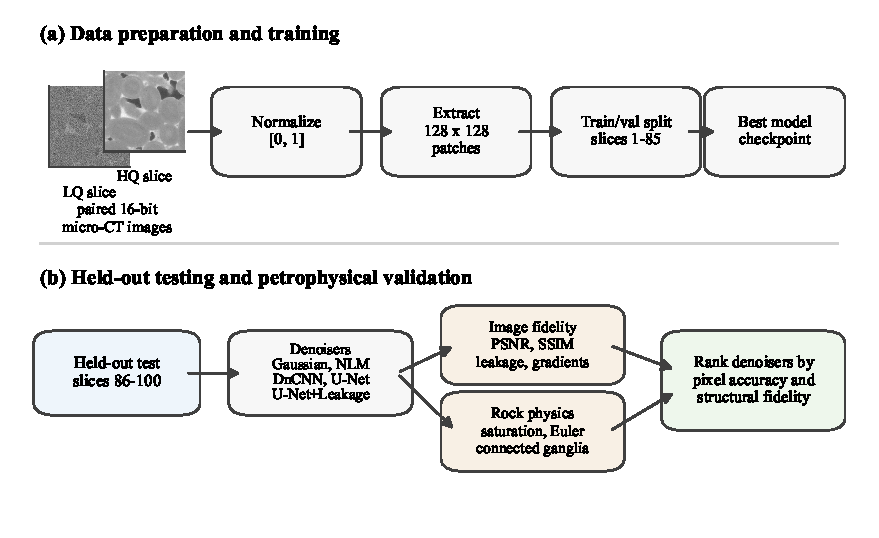
\includegraphics[width=\linewidth]{figures/fig8_full_workflow}
  \caption{End-to-end workflow used in this study.  Paired HQ and LQ
           micro-CT slices are normalized and split into slice-disjoint
           training, validation, and test sets.  Classical filters and
           trained deep denoisers are then evaluated on the same 15
           held-out test slices using image-quality metrics and
           petrophysical descriptors, allowing pixel fidelity to be
           compared directly with structural faithfulness.}
  \label{fig:full_workflow}
\end{figure}

\begin{figure}[ht]
  \centering
  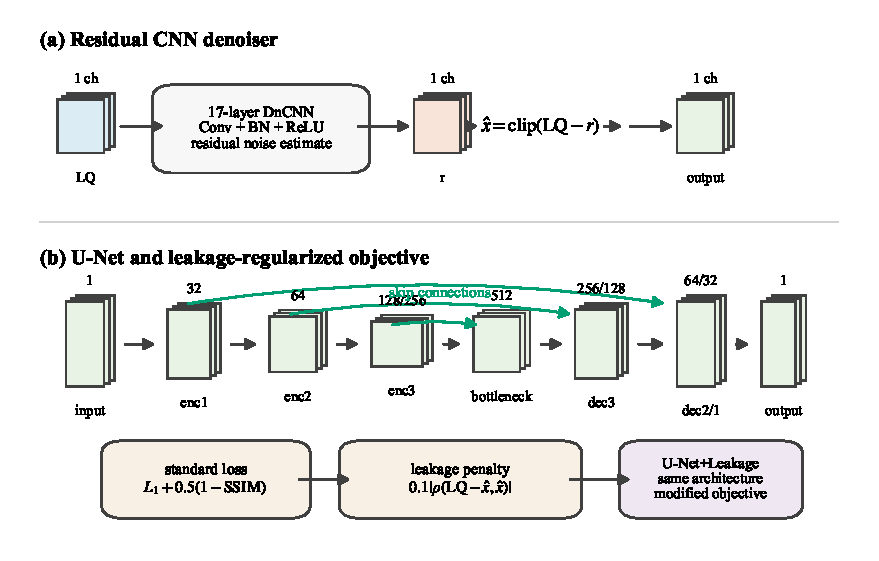
\includegraphics[width=\linewidth]{figures/fig9_architecture_workflow}
  \caption{Architecture and training-objective workflow for the neural
           denoisers.  DnCNN follows a residual path in which the network
           predicts the noise component and subtracts it from the LQ
           input.  U-Net and U-Net+Leakage use the same four-level
           encoder-decoder with skip connections; U-Net+Leakage differs
           only by adding the structural leakage penalty to the standard
           L1--SSIM objective.}
  \label{fig:architecture_workflow}
\end{figure}

\begin{figure}[ht]
  \centering
  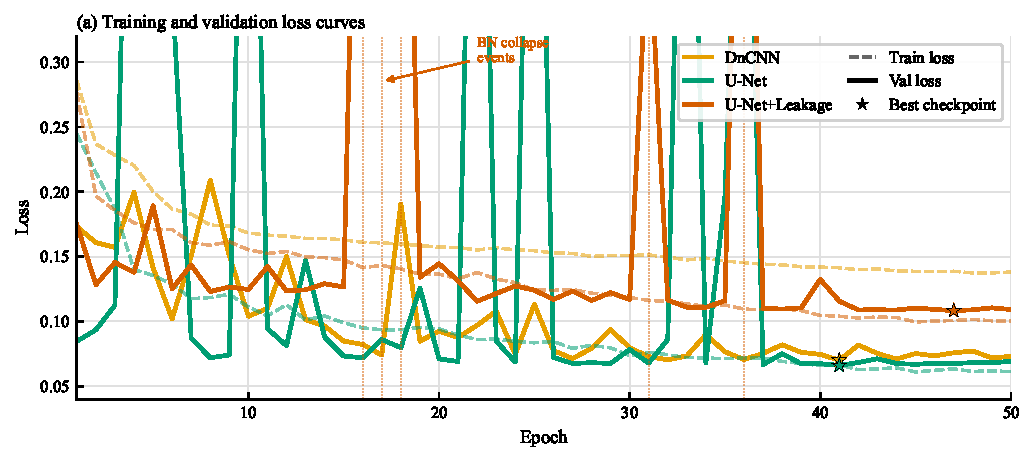
\includegraphics[width=\linewidth]{figures/fig1_training_curves}
  \caption{Validation loss curves for the three deep learning denoisers
           over 50 training epochs.  DnCNN and U-Net converge smoothly
           to best-checkpoint validation losses of 0.0701 and 0.0660,
           respectively.  Three transient spikes to $\approx 0.742$
           are visible in the U-Net+Leakage curve at epochs 16--18, 31,
           and 36, corresponding to batch normalization collapse events.
           In each case the model recovers within three epochs.}
  \label{fig:training_curves}
\end{figure}

\begin{figure}[ht]
  \centering
  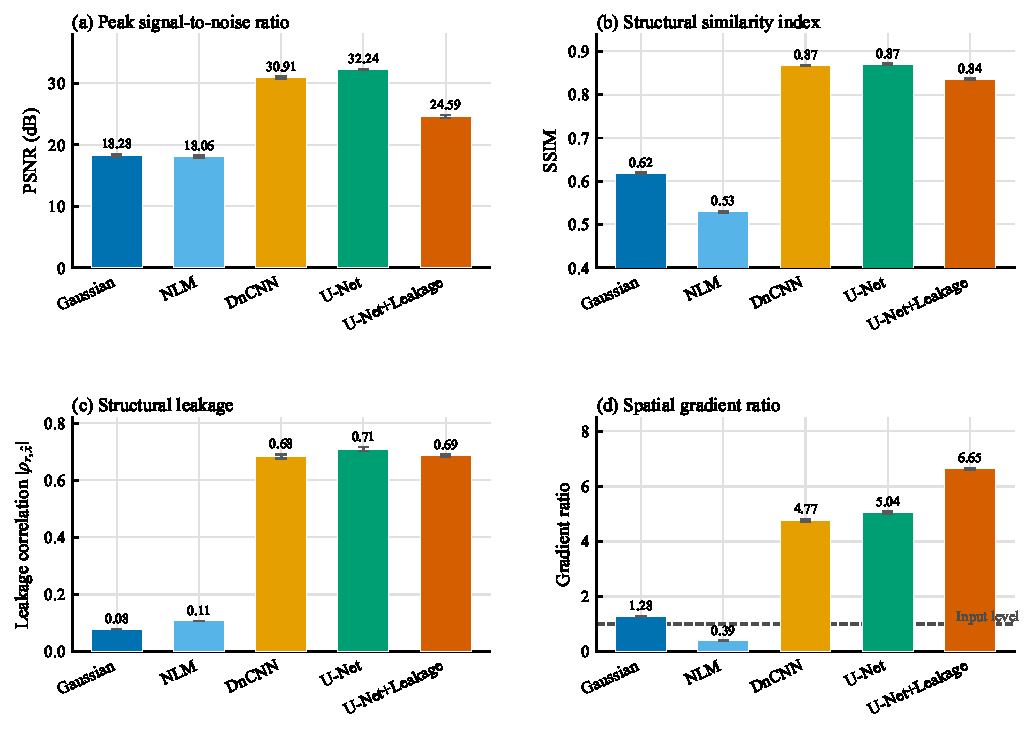
\includegraphics[width=\linewidth]{figures/fig2_image_quality}
  \caption{Image quality metrics for all five denoising methods over
           the 15 test slices (mean $\pm 1$ standard deviation).
           (a)~PSNR and (b)~SSIM show that deep learning methods
           substantially outperform classical filters on pixel-similarity
           measures.  (c)~Structural leakage correlation is six to nine
           times higher for deep learning methods (0.68--0.71) than for
           classical filters (0.08--0.11), indicating that pixel
           fidelity and structural faithfulness are misaligned objectives.
           (d)~Gradient ratio above 1 indicates increased apparent
           sharpness relative to the noisy input; U-Net+Leakage produces
           the strongest sharpening (6.65) despite removing the least
           total signal energy.}
  \label{fig:quality_bars}
\end{figure}

\begin{figure}[ht]
  \centering
  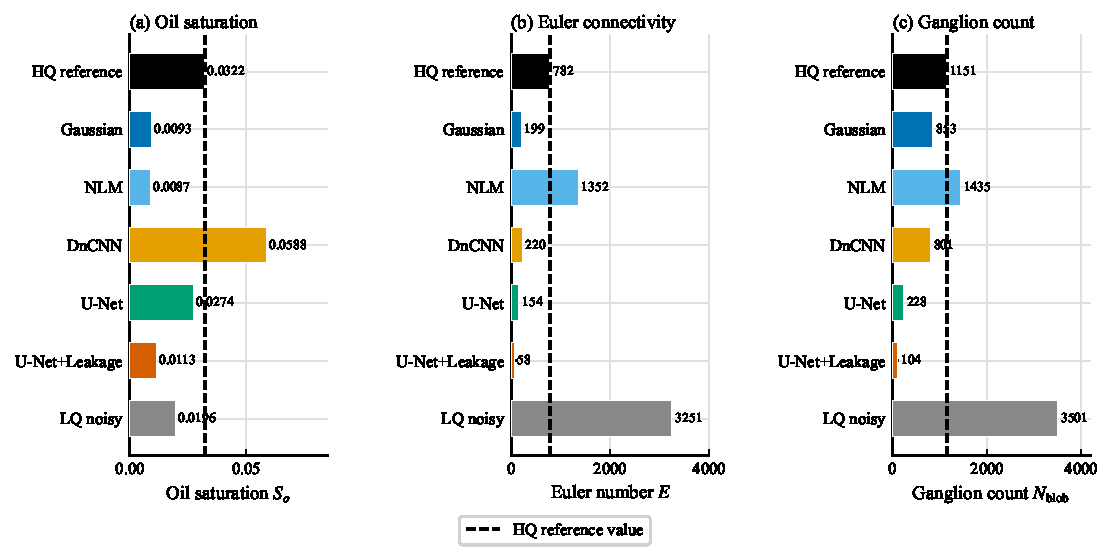
\includegraphics[width=\linewidth]{figures/fig3_petrophysics}
  \caption{Petrophysical metrics for all five denoising methods
           compared with the clean-scan HQ reference and the unprocessed
           LQ noisy input (mean over 15 test slices; dashed vertical
           line marks the HQ reference value).
           (a)~Oil saturation $S_o$: U-Net most closely matches the
           reference (error 15\%); DnCNN overestimates (error 83\%);
           U-Net+Leakage underestimates (error 65\%).
           (b)~Euler connectivity number $E$: all three deep learning
           methods reduce connectivity by 72--93\% relative to the
           reference of 782.
           (c)~Ganglion count $N_{\mathrm{blob}}$: DnCNN retains the
           most ganglia (70\% retention); U-Net+Leakage retains the
           fewest (9\%).}
  \label{fig:euler}
\end{figure}

\begin{figure}[ht]
  \centering
  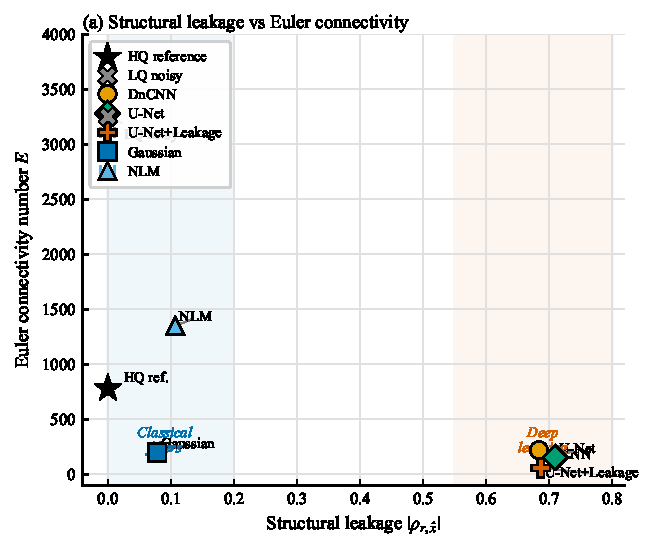
\includegraphics[width=0.75\linewidth]{figures/fig4_leakage_vs_euler}
  \caption{Structural leakage correlation vs.\ Euler connectivity
           number for all five denoisers.  Classical filters (squares)
           cluster at low leakage and Euler numbers closer to the
           clean reference (star).  Deep learning methods (circles)
           cluster at high leakage and severely reduced Euler numbers.
           Within the deep learning group, the relationship is
           non-monotone: U-Net+Leakage shows the lowest leakage but
           the worst Euler number.}
  \label{fig:leakage_vs_euler}
\end{figure}

\begin{figure}[ht]
  \centering
  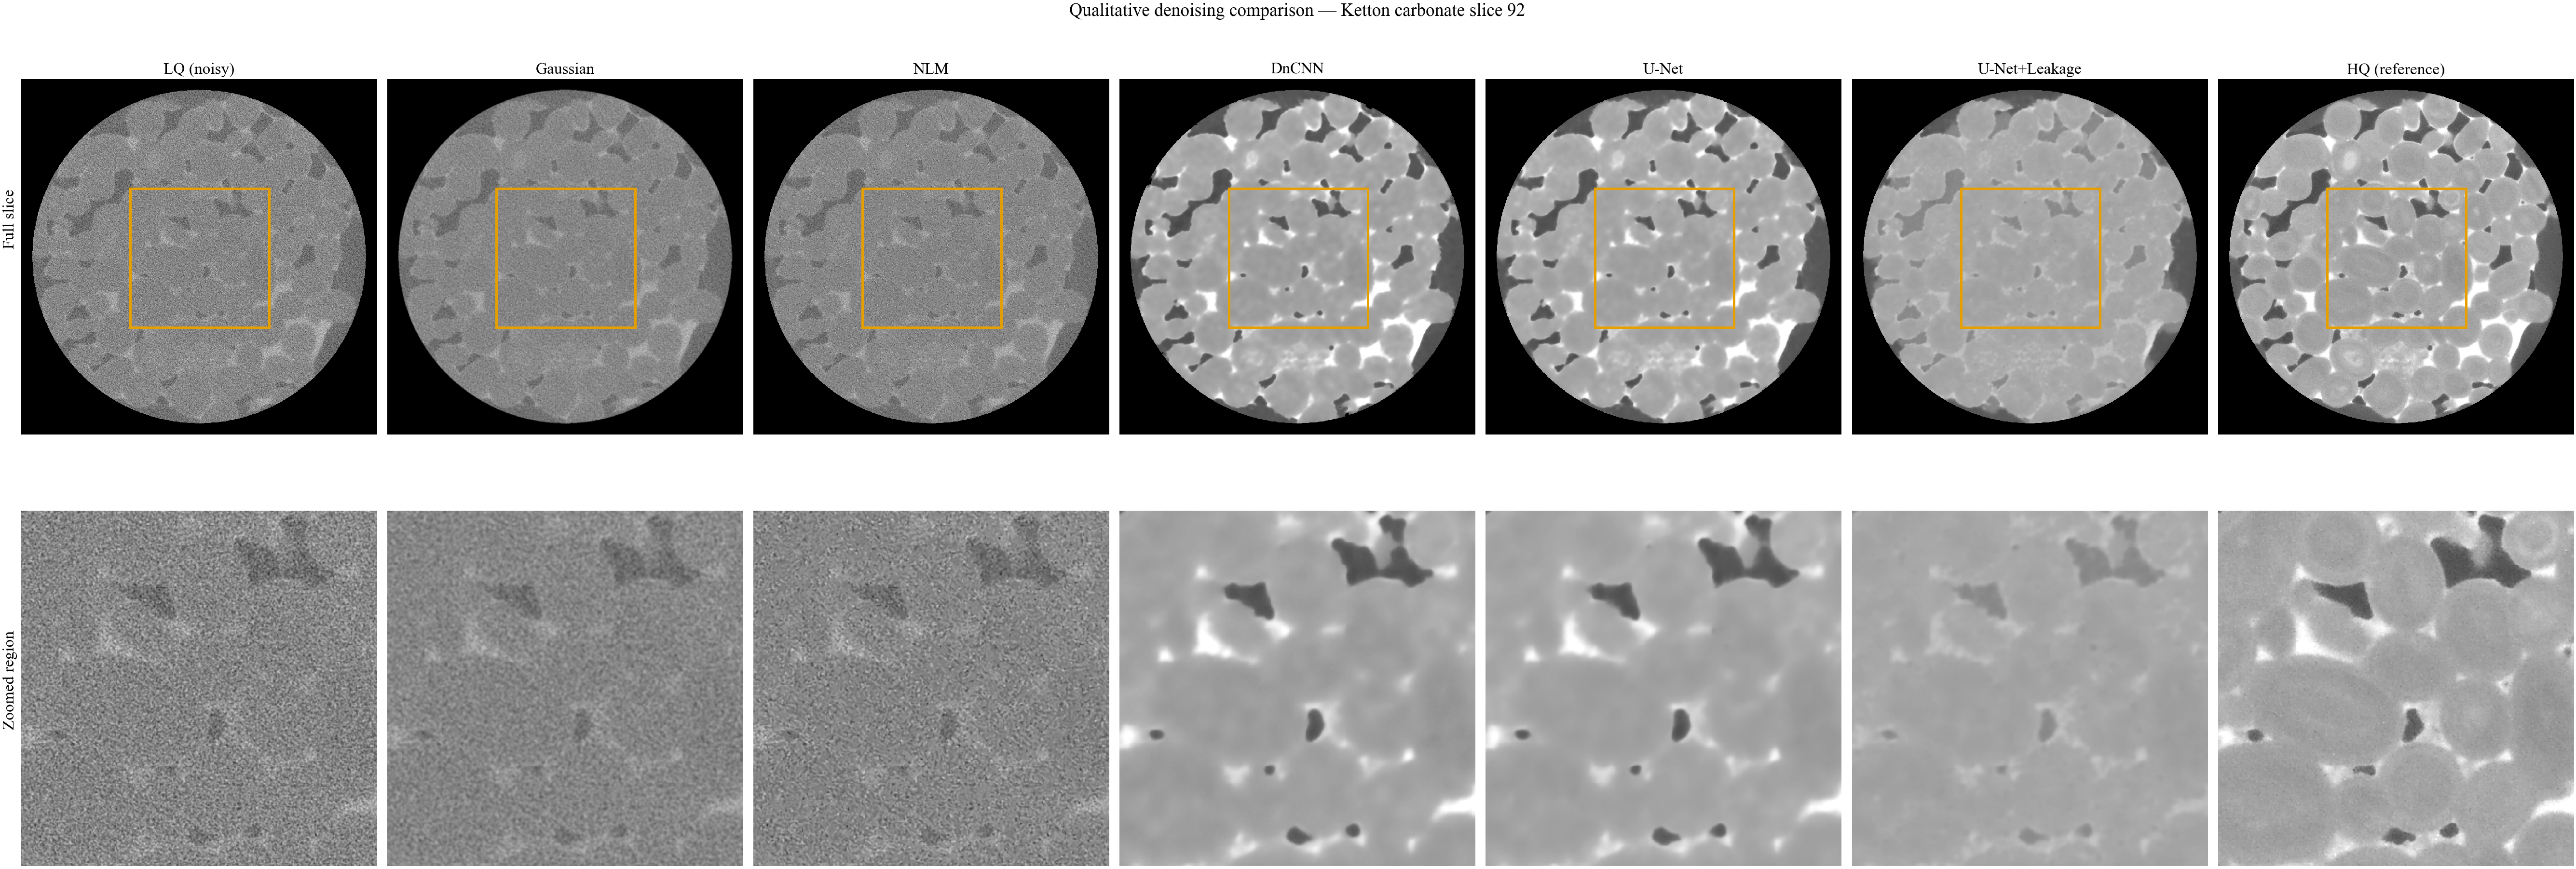
\includegraphics[width=\linewidth]{figures/fig_visual_comparison}
  \caption{Qualitative denoising comparison on representative test
           slice~92.  Top row: full $1024\times1024$ slice for each
           method; bottom row: $400\times400$ zoom of the pore-rich
           central region (orange box).  Gaussian and NLM preserve
           grain boundaries but leave residual granular noise.  DnCNN,
           U-Net, and U-Net+Leakage suppress noise visually but merge
           fine oil ganglia and smooth pore throats relative to the HQ
           reference (green border).  These structural losses are
           quantified by the Euler-number data in
           Table~\ref{tab:physics}.}
  \label{fig:qualitative_zoom}
\end{figure}

\begin{figure}[ht]
  \centering
  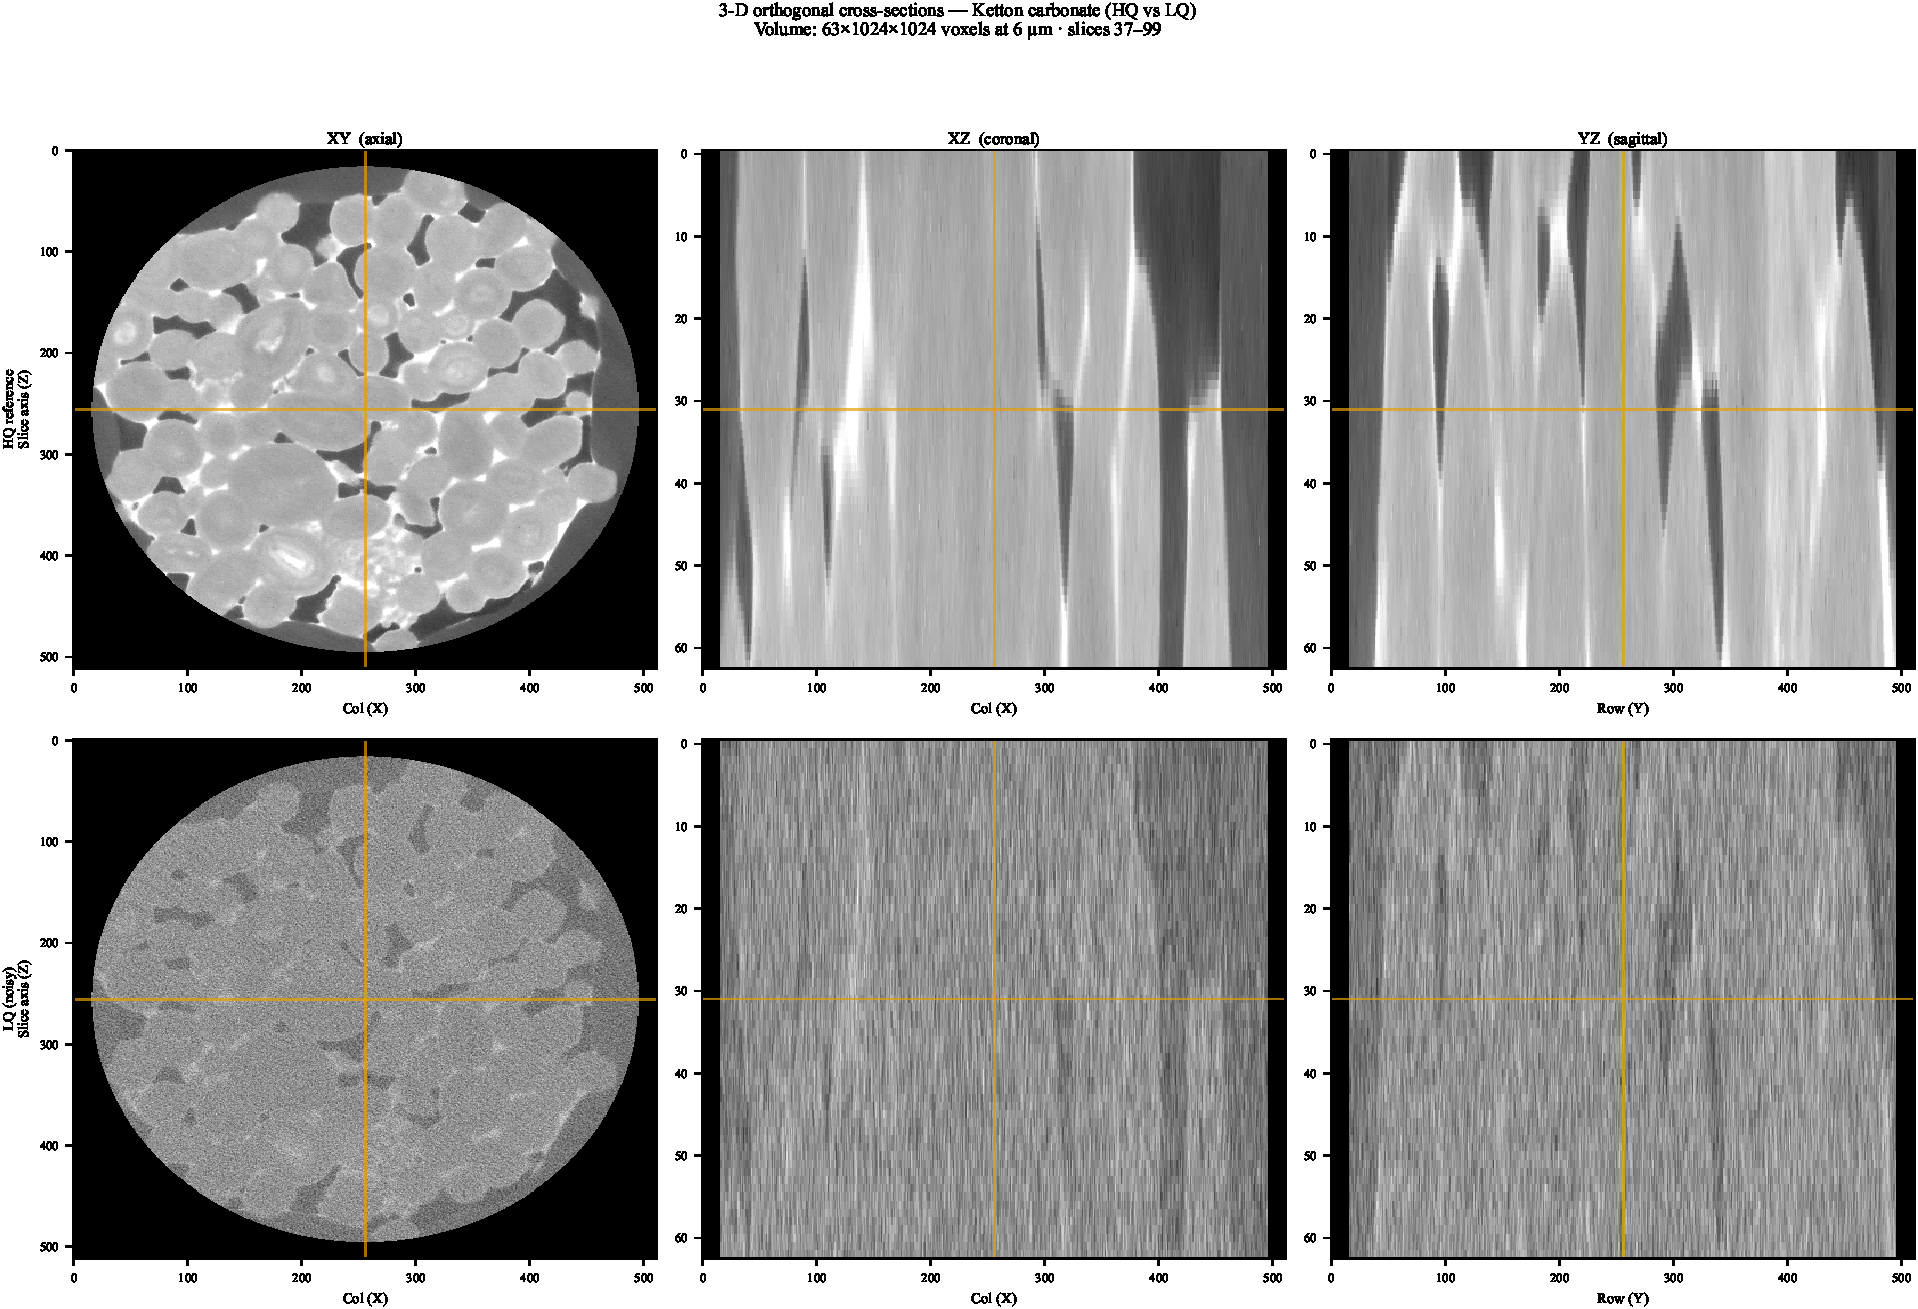
\includegraphics[width=\linewidth]{figures/fig_3d_ortho}
  \caption{Three-dimensional orthogonal cross-sections of the Ketton
           carbonate volume (63 slices, indices 37--99; voxel size
           6~\si{\micro\metre}).  Each row shows the HQ reference (top)
           and LQ fast-acquisition (bottom) volumes in the axial (XY),
           coronal (XZ), and sagittal (YZ) planes.  Orange cross-hairs
           mark the mid-volume intersection.  The LQ planes show
           pronounced reconstruction noise relative to the HQ
           reference, motivating the denoising pipeline evaluated in
           this study.}
  \label{fig:3d_ortho}
\end{figure}

\begin{figure}[ht]
  \centering
  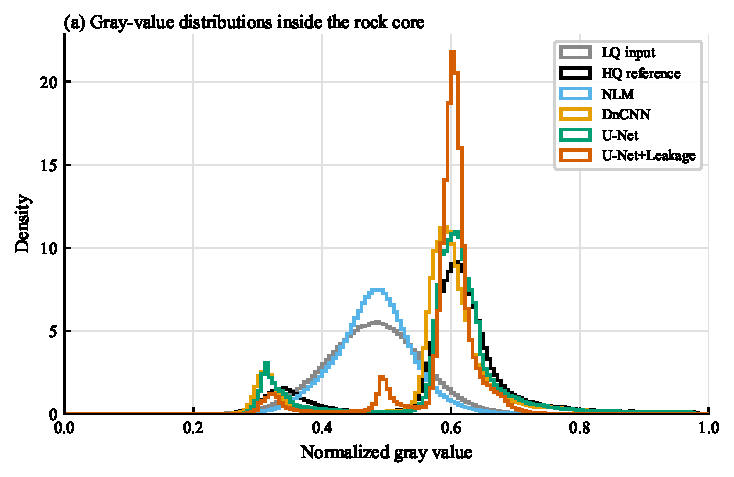
\includegraphics[width=0.78\linewidth]{figures/fig6_gray_histograms}
  \caption{Gray-value distributions inside the rock core for
           representative test slice 92.  The LQ input has a broad
           low-contrast distribution, while the HQ reference has a more
           separated high-intensity mode.  Deep learning methods sharpen
           or shift the high-intensity mode, indicating that good
           pixel-level metrics do not necessarily preserve the same
           intensity distribution as the clean reference.}
  \label{fig:gray_histograms}
\end{figure}

\begin{figure}[ht]
  \centering
  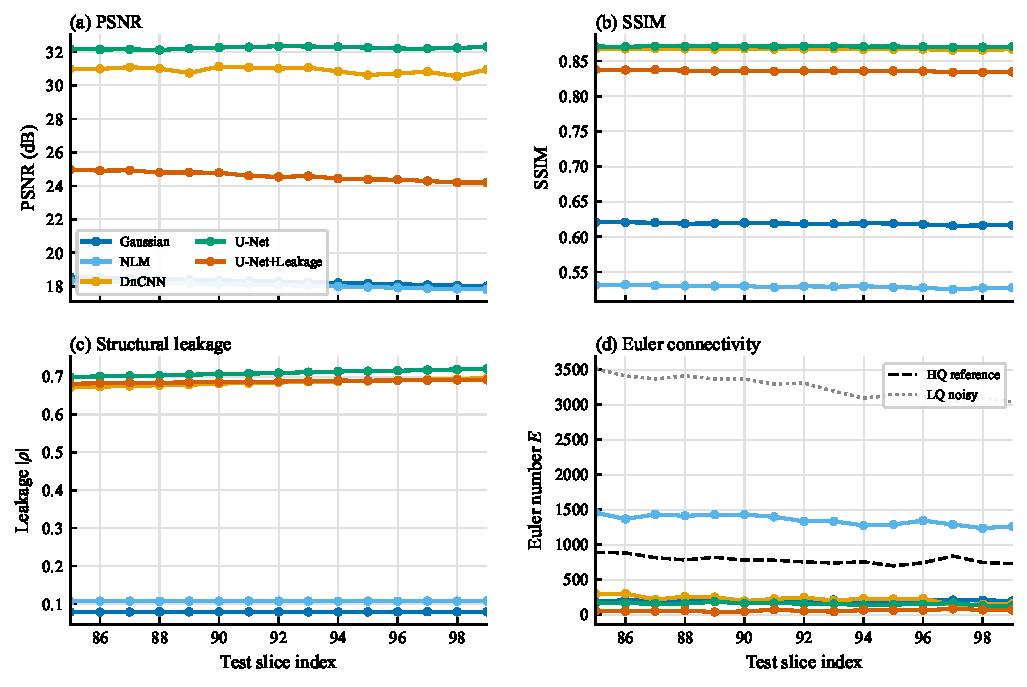
\includegraphics[width=\linewidth]{figures/fig7_slice_trends}
  \caption{Per-slice image-quality and petrophysical trends across the
           15 held-out test slices.  PSNR and SSIM remain stable for
           each method, and structural leakage consistently separates
           classical filters from deep learning denoisers.  Euler
           connectivity remains far below the HQ reference for all
           three deep learning methods across the full test interval,
           showing that the topology loss is systematic rather than
           slice-specific.}
  \label{fig:slice_trends}
\end{figure}

\begin{figure}[ht]
  \centering
  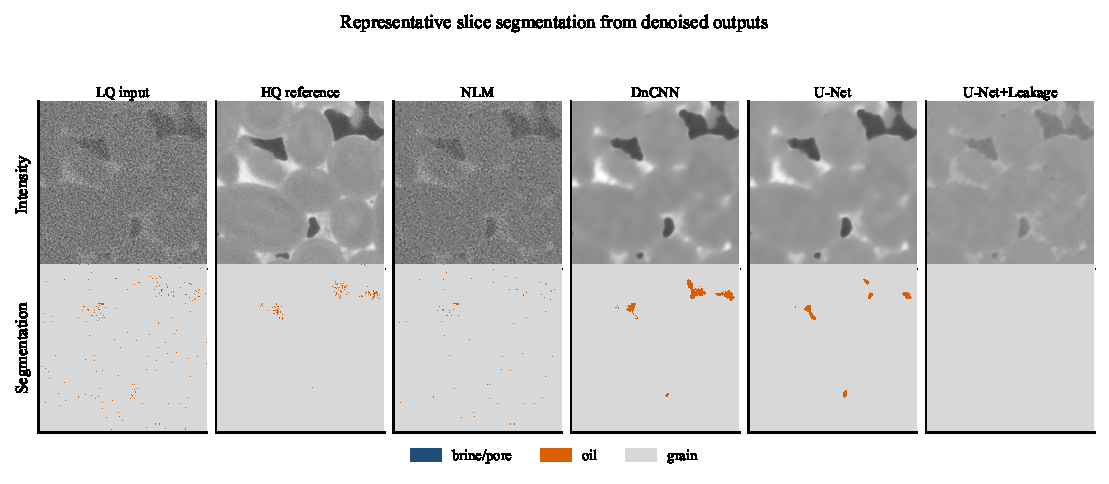
\includegraphics[width=\linewidth]{figures/fig10_segmentation_comparison}
  \caption{Segmentation comparison for representative test slice 92,
           following the qualitative style of dynamic CT denoising
           result figures.  The top row shows cropped intensity images,
           and the bottom row shows the corresponding three-phase
           segmentation into brine/pore, oil, and grain.  Differences
           in the segmented oil phase reveal how denoising changes the
           downstream petrophysical interpretation even when the
           intensity image appears visually smooth.}
  \label{fig:segmentation_comparison}
\end{figure}

\begin{figure}[ht]
  \centering
  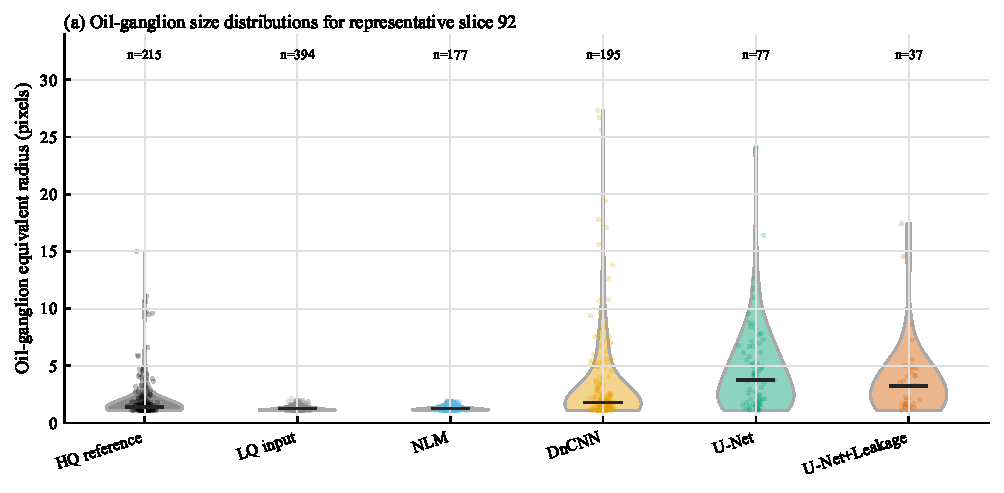
\includegraphics[width=0.88\linewidth]{figures/fig11_ganglion_distribution}
  \caption{Oil-ganglion equivalent-radius distributions for
           representative test slice 92.  The distributions are computed
           from connected components in the segmented oil phase.  Deep
           learning denoisers reduce the number and spread of small oil
           ganglia relative to the HQ reference, consistent with the
           topology loss measured by Euler number and ganglion count.}
  \label{fig:ganglion_distribution}
\end{figure}

\begin{figure}[ht]
  \centering
  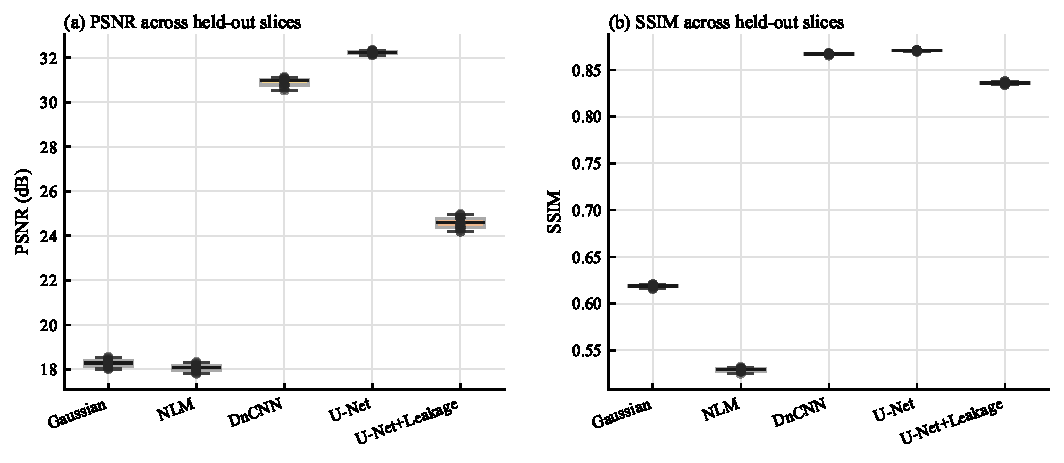
\includegraphics[width=0.95\linewidth]{figures/fig12_metric_distributions}
  \caption{PSNR and SSIM distributions across the 15 held-out test
           slices.  Each point is one test slice and each box summarizes
           the slice-to-slice variation for a denoising method.  The
           deep learning methods dominate PSNR and SSIM, while the
           petrophysical figures show that these image-quality gains do
           not guarantee preservation of oil-phase topology.}
  \label{fig:metric_distributions}
\end{figure}

% ============================================================
\clearpage
\bibliography{paper}

\end{document}
